\documentclass[crop,tikz]{standalone}
\usetikzlibrary{%
    arrows,
    arrows.meta,
    automata,
    backgrounds,
    calc,
    decorations.pathreplacing,
    fit,
    matrix,
    positioning,
    scopes,
    shadows
}
\usepackage[linguistics]{forest}
\usepackage[charter]{mathdesign}
\tikzset{headarrow/.style = {-{Latex[length=.5em]}}}

\begin{document}
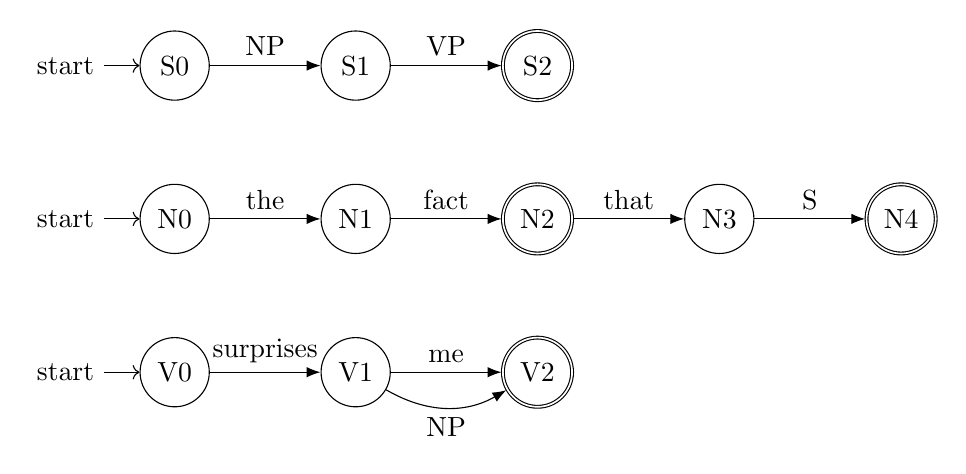
\begin{tikzpicture}
    % automata starts
    \node[state,initial] (S0) at (0,0) {S0};
    \node[state,initial] (N0) [below=3em of S0] {N0};
    \node[state,initial] (V0) [below=3em of N0] {V0};

    % other states
    \foreach \Aut in {S,N,V}
        {
        \node[state]           (\Aut1) [right=4em of \Aut0]  {\Aut1};
        \node[state,accepting] (\Aut2) [right=4em of \Aut1]  {\Aut2};
        }

    % add center embedding
    \node[state] (N3) [right=4em of N2] {N3};
    \node[state,accepting] (N4) [right=4em of N3] {N4};

    % edges
    \foreach \Source/\Target/\Label in {%
        S0/S1/NP,
        S1/S2/VP,
        N0/N1/the,
        N1/N2/fact,
        N2/N3/that,
        N3/N4/S,
        V0/V1/surprises,
        V1/V2/me%
        }
        \draw[headarrow] (\Source) to node [above] {\Label} (\Target);

    % add NP edge
    \draw[headarrow, bend right] (V1) to node[below] {NP} (V2);
\end{tikzpicture}
\end{document}
